\documentclass[12pt]{article}
%\usepackage[utf8]{inputenc}
%\documentclass[UTF8]{ctexart}
%\usepackage[UTF8, heading = false, scheme = plain]{ctex}
\usepackage{geometry}
%geometry{a4paper,scale=0.9}
\geometry{a4paper,left=1cm,right=1cm,top=1cm,bottom=2cm}
\usepackage{amsfonts}
\usepackage{color}
\usepackage{url}
%\usepackage{biblatex}
\usepackage{amsmath}
\usepackage{amssymb}
\usepackage{latexsym}
\usepackage{cite}
%\addbibresource{ref.bib}
%\bibliography{ref.bib}
\usepackage{caption}
\usepackage{graphicx, subfig}
\usepackage{float}
%\usepackage[fontset=ubuntu]{ctex}
%\usepackage{fontspec}
\usepackage{xeCJK}
%\usepackage[colorlinks,
%anchorcolor=black,
%citecolor=black]{hyperref}
%\setmainfont{SimSun}
\usepackage[section]{placeins}
\usepackage{enumitem}
\usepackage{framed}
\usepackage[framemethod=TikZ]{mdframed}
\usepackage{indentfirst}
\usepackage{setspace}%使用间距宏包
\linespread{1.5}
%\title{预备知识}
%\author{leolinuxer }
%\date{June 2020}

\title{概率统计基础知识\cite{Common_Probability_Distribution}\cite{Inference_Of_Expectation_Variations}}
%\author{leolinuxer }
%\date{June 2020}

\begin{document}
%\setlength{\parindent}{0pt}
\maketitle
\tableofcontents

\section{基础定义}
\subsection{统计相关的基础知识}
横断面研究(cross-sectional study):研究某个时间点下样本的情况

纵贯研究(longitudinal study):在一段时间内反复观察同一批样本\cite{Think_Stats}

\subsection{随机变量}
随机变量是可以随机地取不同值的变量。例如:抛掷一枚硬币,出现正面或者反面的结果;从一个班级中,随机选一个同学,他的身高值。

\textbf{随机变量可以是离散的或者连续的}。离散随机变量拥有有限(例如正面或者反面)或者可数无限多的状态。连续随机变量伴随着实数值(例如:身高)。

\subsection{概率质量函数和概率密度函数}
\textbf{离散型变量的概率分布可以用概率质量函数(Probability Mass Function,简称PMF)来描述}。我们通常用大写字母P来表示概率质量函数。

\textbf{当研究的对象是连续型随机变量时,我们用概率密度函数(Probability Density Function,简称PDF)来描述它的概率分布}。我们通常用小写字母p来描述概率密度函数。

\subsection{期望}
函数 $f(x)$ 关于某分布的期望(Expectation)或者期望值(Expected value)是指:当x由P产生,f作用于x时,$f(x)$的平均值。

对于离散型随机变量,期望值可以通过求和得到:
$$
E_{x \sim P[f(x)]} = \sum_xP(x)f(x)
$$

对于连续型随机变量,期望值可以通过求积分得到:
$$
E_{x \sim p[f(x)]} = \int p(x)f(x) dx
$$

\subsection{方差与标准差}
方差(Variance)衡量的是当我们对x依据它的概率分布进行采样时,随机变量x的函数值会呈现多大的差异。计算方差的函数如下:
$$
Var(f(x)) = E[(f(x)-E[f(x)])^2]
$$
方差的平方根称之为标准差(Standard Deviation)。有些资料也称标准差为均方差。

设有一个随机变量$X$, 其期望存在为$E(X)$,方差存在为$D(X)$,那么有结论:
$$
D(X) = E(X^2) - [E(X)]^2
$$

其中,$E(X^2)$ 是 $X^2$ 的期望。

例如,已知 $P(X=1)= 2/3, P(X=0) = 1/6, P(X=-1) = 1/6$,那么:

$$
E(X) = 1 * 2/3 + 0 * 1/6 +(-1) * 1/6 = 2/3 - 1/6 = 1/2
$$

$$
E(X^2) = 1^2 * 2/3 + 0^2 * 1/6 + (-1)^2 * 1/6 = 2/3 + 1/6 = 5/6.
$$

$$
D(X) = E(X^2) - [E(X)]^2 = 5/6 - (1/2)^2 = 7/12
$$


\subsubsection{一幅图理解期望和方差}
台湾大学李毅宏教授的这节课程: 《Where does the error come from?》 仅仅通过一幅图就非常好的解释了期望和方差的概念。

结果与期望的偏离称之为偏差(Bias)。通俗的讲,Bias描述了结果与中心的偏离程度。而方差(Variance)描述了结果互相之间的散列程度。

你可以对比下面这幅图的四种情况来加深理解:
\begin{figure}[ht]
  \centering
  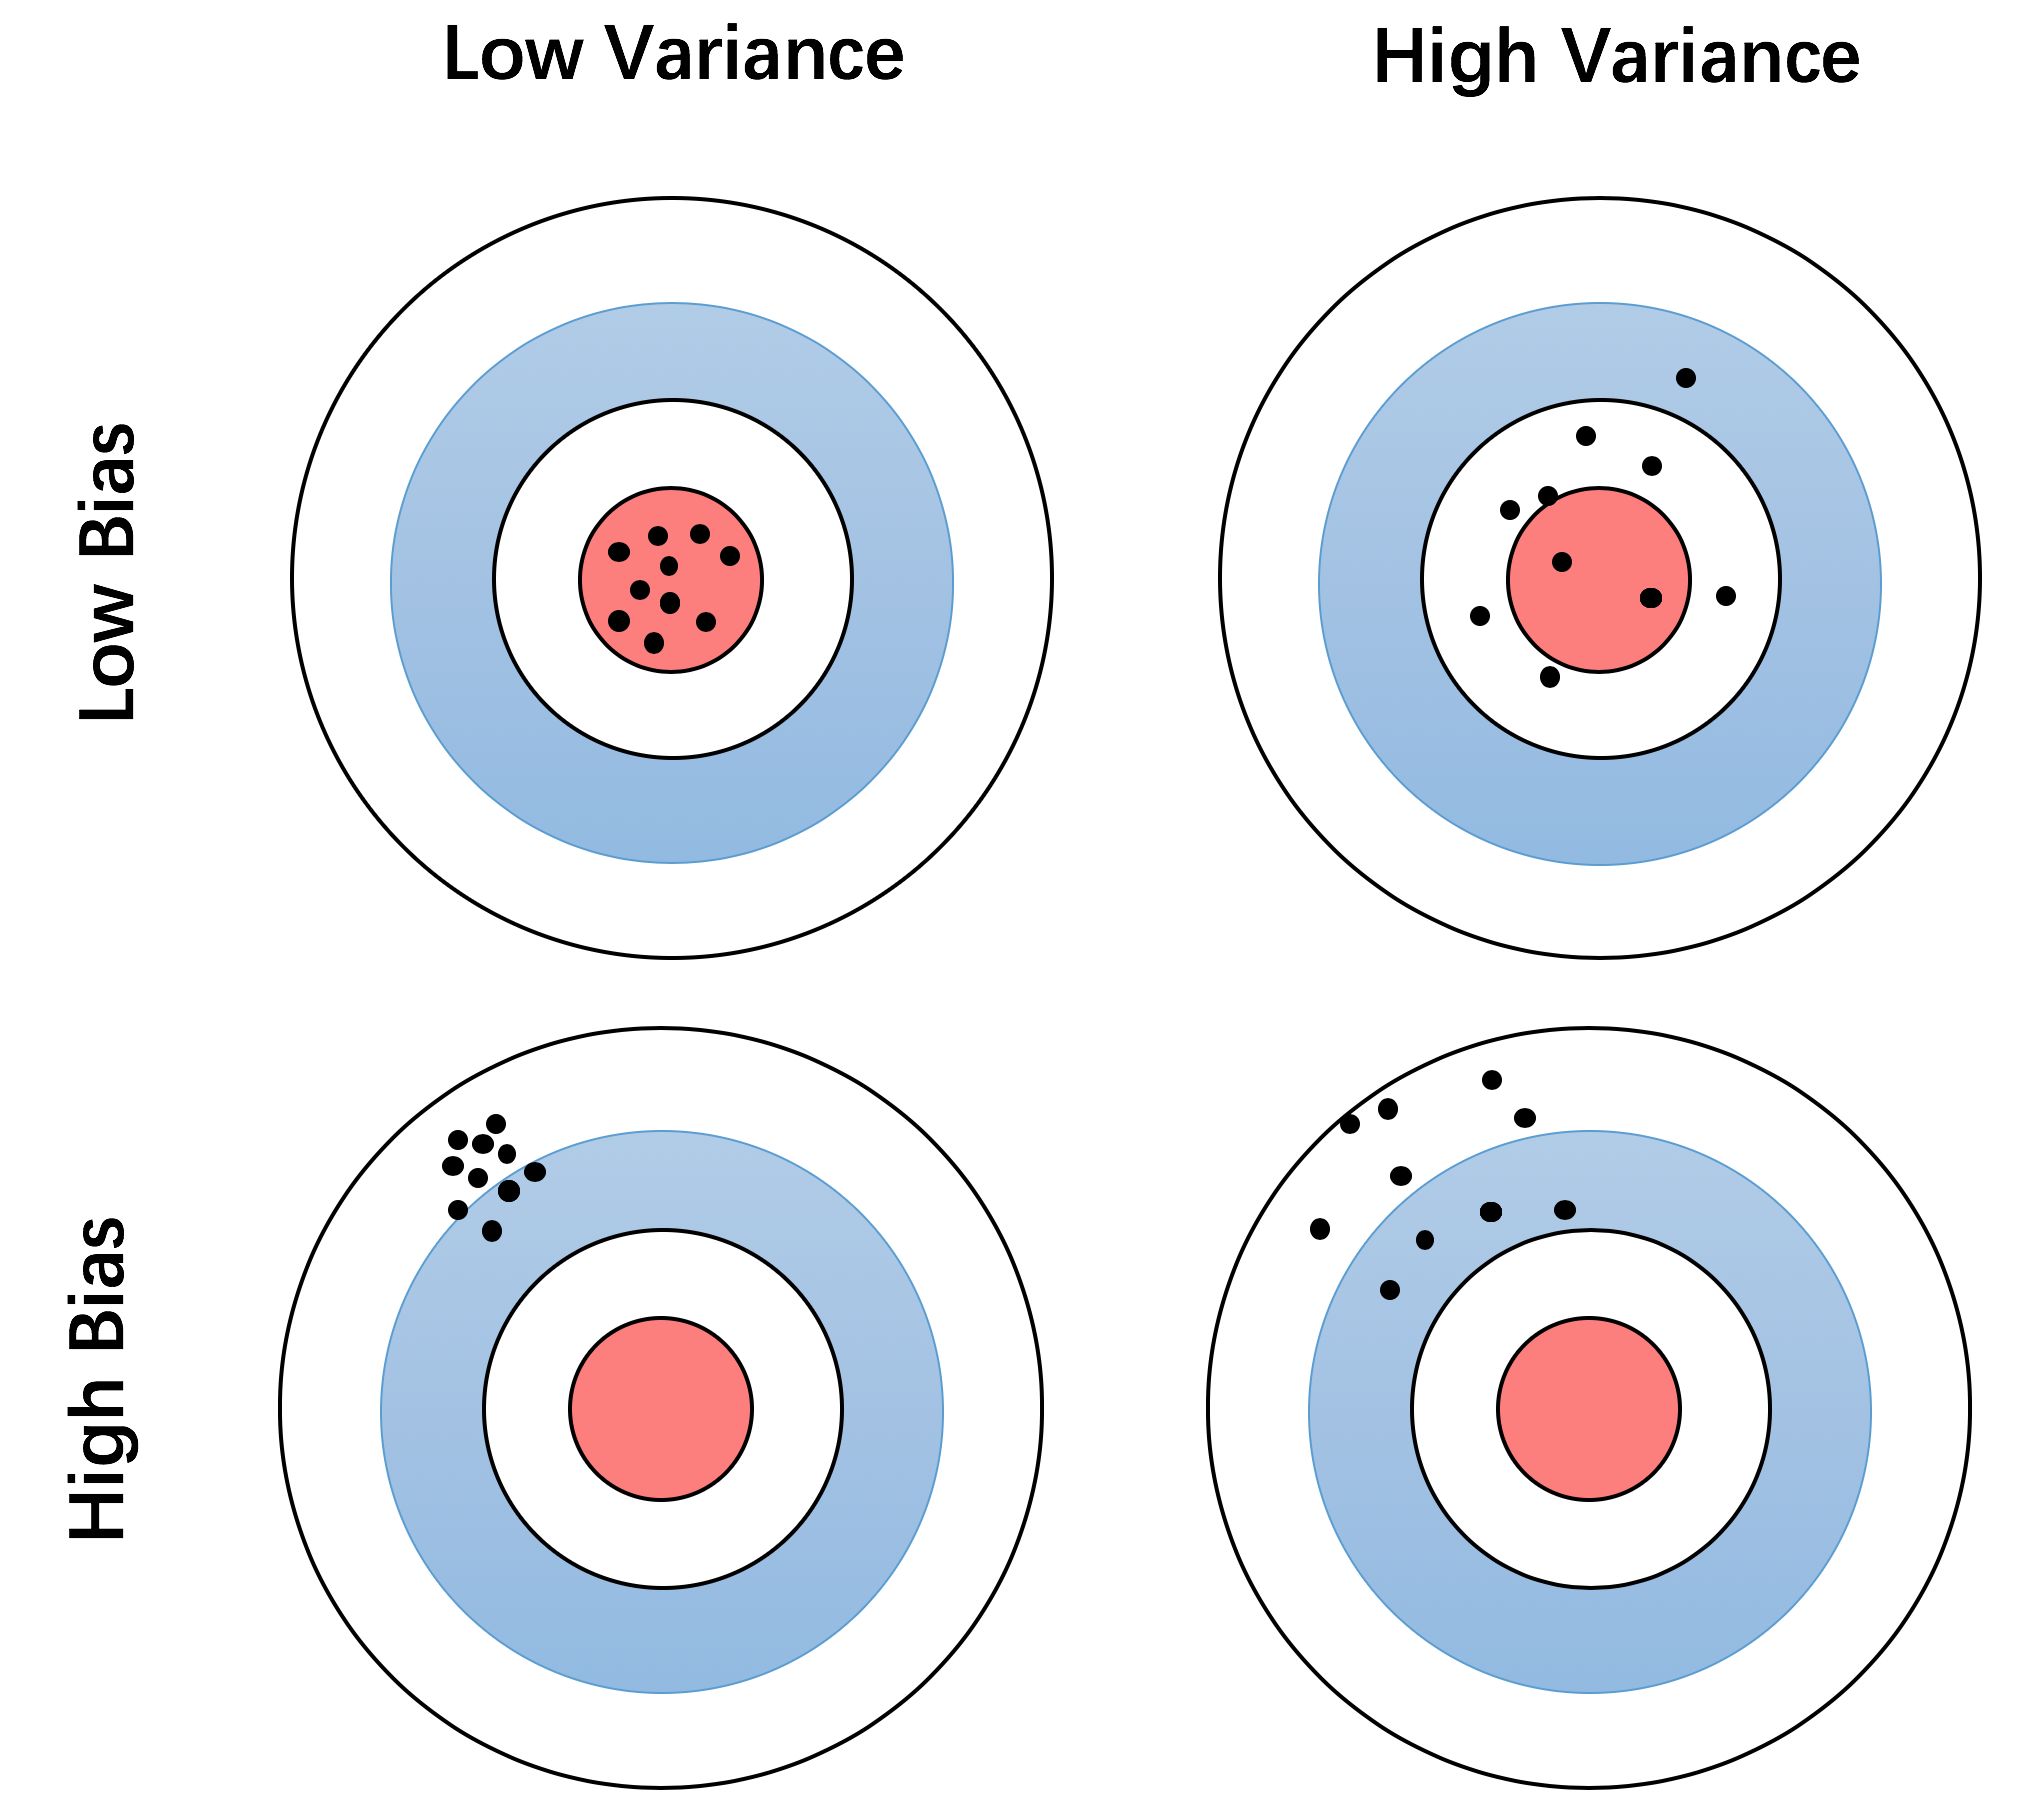
\includegraphics[width=.8\textwidth]{fig/bias_variance.png} %1.png是图片文件的相对路径
  \caption{Bias 和方差的比较} %caption是图片的标题
  %\label{HingeLossExample} %此处的label相当于一个图片的专属标志,目的是方便上下文的引用
\end{figure}

从这幅图中我们可以看出:
\begin{itemize}
    \item 当Bias和Variance都比较小的时候,结果都比较紧密的集中在预期的值上。
    \item 当Bias较小而Variance较大时,意味着结果较靠近预期,但是比较散落。
    \item 当Bias较大而Variance较小时,意味着结果集中在一起,但是离预期值偏离较多。
    \item 当Bias和Variance都较大时,意味着结果既不靠近预期,也比较散落。
\end{itemize}

\subsubsection{凸函数和Jensen不等式\cite{Understanding_Jensen_Nnequality_And_Proof}}
\textbf{凸函数}

凸函数是一个定义在某个向量空间的凸子集 $C$(区间)上的实值函数 $f$,如果在其定义域 $C$ 上的任意两点 $x1,x2x $, $0 \le t \le 1 $ ,有
$$
tf(x_1) + (1-t)f(x_2) \ge f(tx_1 + (1-t)x_2)
$$

就是说凸函数任意两点的割线位于函数图形上方, 这也是\textbf{Jensen不等式的两点形式}。

\textbf{Jensen不等式}

若对于任意点集$\{xi\}$,若$\lambda_i \ge 0$ 且$\sum_i\lambda_i = 1$,则凸函数 $f(x)$ 满足:
$$
f(\sum_{i=1}^{M}\lambda_ix_i) \le \sum_{i=1}^{M}\lambda_if(x_i)
$$

\begin{framed}  
%\verb|\documentstyle[ifthen,12pt,titlepage]{article}|
\small{
使用数学归纳法证明如下:

当 $i=1$或 $i=2$时,根据凸函数的定义,显然成立;

假设当 $i=M$ 时不等式成立,现在证明当 $i=M+1$ 时不等式也成立:
\begin{align*}
f(\sum_{i=1}^{M+1}\lambda_ix_i) &= f(\lambda_{M+1}x_{M+1} + \sum_{i=1}^M\lambda_ix_i) \\
&= f(\lambda_{M+1}x_{M+1} + (1-\lambda_{M+1})\sum_{i=1}^M\eta_ix_i)
\end{align*}
其中,
$$
\eta_i = \frac{\lambda_i}{1 - \lambda_{M+1}}
$$

注意到 $\lambda_i$ 满足:
$$
\sum_{i=1}^{M+1}\lambda_i = 1
$$

所以:
$$
\sum_{i=1}^{M}\lambda_i = 1 - \lambda_{M+1}
$$

所以$\eta_i$ 满足:
$$
\sum_{i=1}^{M}\eta_i = \frac{\sum_{i=1}^{M}\lambda_i }{1 - \lambda_{M+1}} = 1
$$

所以:
$$
\sum_{i=1}^{M}f(\eta_ix_i) \le \sum_{i=1}^{M}\eta_if(x_i)
$$

所以命题得证:
$$
f(\sum_{i=1}^{M+1}\lambda_ix_i) \le \lambda_{M+1}f(x_{M+1}) + (1-\lambda-{M+1})\sum_{i=1}^{M}\eta_if(x_i) = \sum_{i=1}^{M+1}\lambda_if(x_i)
$$
}
\end{framed}

\subsubsection{Jensen不等式和期望}
\textcolor{red}{在概率论中,如果把$λ_i$ 看成取值为 $x_i$的离散变量 $x$ 的概率分布,那么 Jensen不等式就可以写成:}
$$
f(E[x]) \le E[f(x)]
$$

对于连续变量,Jensen不等式给出了积分的凸函数值和凸函数的积分值间的关系:
$$
f(\int{xp(x)dx}) \le \int{f(x)p(x)dx}
$$

\begin{framed}  
%\verb|\documentstyle[ifthen,12pt,titlepage]{article}|
\small{
一道关于概率论的不等式问题:已知 $X_1, X_2, X_3>0$是某个概率空间上的随机变量,证明:
$$
E[\frac{X_1}{X_2}]E[\frac{X_2}{X_3}]E[\frac{X_3}{X_1}] \ge 1
$$

证明:先看有两个变量的情况:

令$g(x) = \frac{1}{x}, \quad x > 0$,则 $g(x)$是右半空间上的凸函数。所以根据 Jensen 不等式,有:
$$
E[g(x)] \ge g(E[x]) = \frac{1}{E[x]}
$$

令 $x = \frac{X_1}{X_2}$,则有:
$$
E[g(\frac{X_1}{X_2})] \ge g(E[\frac{X_1}{X_2}]) = \frac{1}{E[\frac{X_1}{X_2}]}
$$
$$
E[\frac{X_1}{X_2}]E[g(\frac{X_1}{X_2})] \ge E[\frac{X_1}{X_2}]\frac{1}{E[\frac{X_1}{X_2}]} = 1
$$

更进一步,有(??如何证明??):
$$
E[\frac{X_1}{X_3}] = E[\frac{X_1}{X_2}\frac{X_2}{X_3}] \le E[\frac{X_1}{X_2}]E[\frac{X_2}{X_3}]
$$

那么对于三个元的情况类似得可以按以下方式处理,
$$
E[\frac{X_1}{X_2}]E[\frac{X_2}{X_3}]E[\frac{X_3}{X_1}] \ge E[\frac{X_1}{X_3}]E[\frac{X_3}{X_1}] = \ge 1
$$
}
\end{framed}

\subsubsection{期望和协方差的关系}
\begin{align*}
Cov(X,Y) &= E[X - E[X]]\cdot E[Y-E[Y]] \\
    &= E[XY] - E[XE[Y]+YE[X]] + E[E[X]E[Y]] \\
    &= E[XY] - 2E[X]E[Y] + E[X]E[Y] \\
    &= E[XY] - E[X]E[Y]
\end{align*}

\subsubsection{偏度(skewness)和皮尔逊中值偏度系数(Pearson's median skewness coefficient)\cite{Think_Stats}}
\textbf{偏度}是度量分布函数不对称程度的统计量。对于一个给定的序列 $x_i$,样本偏度的定义为:
$$
g_1 = m_3 / m_2^{\frac{3}{2}}
$$
$$
m_2 = \frac{1}{n}\sum_i(x_i - \mu)^2
$$
$$
m_3 = \frac{1}{n}\sum_i(x_i - \mu)^3
$$

负的偏度表示分布向左偏,此时分布函数的左边会比右边延伸的更长;正的偏度表示分布函数向右偏。

偏度受异常值的影响比较大。更好的比较方式是比较均值和中位数的大小。因为均值更容易受到极端值的影响,但是中位数不易受到影响。

\textbf{皮尔逊中值偏度系数}的定义如下:
$$
g_p = 3(\mu - \mu_{\frac{1}{2}})/\sigma
$$

其中,$\mu$ 为均值,$\mu_{\frac{1}{2}}$ 为中位数。

皮尔逊中值偏度系数是偏度的一个鲁邦估计,对异常值的影响不敏感。

\subsection{相关性}
\subsubsection{协方差(Covariance)\cite{Think_Stats}}
协方差用来衡量相关变量的变化趋势是否相同。假设我们有两列序列 $X$ 和 $Y$,他们与其均值的离差为:
$$
dx_i = x_i - \mu_x 
$$
$$
dy_i = y_i - \mu_y
$$

协方差就是这些乘积结果的平均值:
$$
Cov(X,Y) = \frac{1}{n}\sum{dx_idy_i}
$$

$n$ 表示序列的长度($X$和$Y$必须有相同的长度)。

\subsection{皮尔逊相关系数}
$$
p_i = \frac{(x-\mu_x)}{\sigma_x}\frac{(y_i-\mu_y)}{\sigma_y}
$$

皮尔逊相关系数定义为:
$$
\rho = \frac{1}{n}\sum{p_i}
$$

\textbf{相关系数$\rho$的取值为-1到1之间},简单的证明如下:
$$
\rho = \frac{1}{n}\sum{p_i} = \frac{Cov(X,Y)}{\sigma_X\sigma_Y}
$$

将离差项带入公式,有
$$
\rho = \frac{\sum dx_idy_i}{\sum{dx_i}\sum{dy_i}}
$$

利用著名的柯西-施瓦兹不等式(Cauchy-Schwarz innequality)即可证明 $\rho^2 <= 1$,即 $-1 <= \rho <= 1$

$\rho$描述了两个变量相关的程度,当 $\rho = 1$时,两个变量完全相关,即如果我们知道了其中一个变量的值,就可以精确预测另一个变量的值。$\rho = -1$时表示两个变量是完全负相关的。

皮尔逊相关系数受异常值的影响比较大。

\section{离散型分布}
\subsection{伯努利分布(零一分布)}
伯努利(Bernoulli)分布是最基本,也是我们最常见的分布。伯努利分布在生活中非常的常见。例如,抛掷一枚硬币的结果就是符合伯努利分布的:结果只会是正面或者反面。

伯努利分布亦称“零一分布”、“两点分布”:它的结果只会是两种可能性中的一种,且这两种结果互相对立,必居其一。因此,我们也常常称结果是成功的,或者失败的。

\textbf{好几种其他的分布都与伯努利分布有一定的关系。}

假设伯努利实验成功的概率是p,则伯努利分布的概率质量函数如下:
$$
P(X=x) = p^x (1 - p)^{(1-x)},\; X \in {0, 1}
$$

当然,考虑到X只有0和1两种可能,我们也可以直接写成:
$$
P(X=x) =
\begin{cases}
p\;(x=1) \\
1-p\;(x=0)
\end{cases}
$$

伯努利分布的期望值是 $p$,方差是 $p(1−p)$。

\subsection{二项分布}
我们可以很自然的可以将一次伯努利实验扩展到多次,此时其结果符合二项(Binomial)分布。

二项分布的概率质量函数如下:
$$
P(X=k) = \binom{n}{k}p^{k}(1-p)^{n-k}
$$
$$
\binom{n}{k}  = \frac{n!}{k!(n-k)!}
$$

通过这个函数,我们可以计算出在进行n次的伯努利实验中,有k次出现正面结果的概率。

很显然,当n为1时,这个函数和伯努利的概率质量函数是一样的。

二项分布的期望值是$np$,方差是$np(1-p)$。

期望的推导过程:
\begin{align}
    E(X) &= \sum_{k=0}^nP\{X=k\}k \\
    &= \sum_{k=1}^n \binom{n}{k}kp^{k}(1-p)^{n-k} \\
    &= \sum_{k=1}^nnp\binom{n-1}{k-1}p^{k-1}(1-p)^{n-k} \\
    &= np\sum_{k=1}^n\binom{n-1}{k-1}p^{k-1}(1-p)^{n-k} \\
    &= np
\end{align}
这里有两个变换:
$$
\binom{n}{k} = \frac{n!}{k!(n-k)!} = \frac{n}{k}\binom{n-1}{k-1}
$$
$$
\sum_{k=1}^n\binom{n-1}{k-1}p^{k-1}(1-p)^{n-k} = (p+1-p)^{(n-1)} = 1
$$
\begin{framed}  
%\verb|\documentstyle[ifthen,12pt,titlepage]{article}|
附:该式的推导,已知二次函数
$$
(a+b)^{n-1} = \sum_{i=0}^{n-1}\binom{n-1}{i}b^{n-1-i}a^i
$$

可以看出来,$i \in \{0, 1, \cdots, n-1\}$

令 $k=i+1$,所以 $k \in \{1, 2, \cdots, n\}$,且有:
$$
(a+b)^{n-1} = \sum_{k=1}^{n-1}\binom{n-1}{k-1}b^{n-k}a^{k-1}
$$

进一步可以推导出:
$$
(a+b)^{n-2} = \sum_{k=2}^{n-2} \binom{n-2}{k-2}b^{n-k}a^{k-2}
$$
\end{framed}  

方差的推导过程:
\begin{align}
    E(X^2) &= \sum_{k=0}^n k^2\binom{n}{k}p^k(1-p)^{n-k}  \quad \text{令 1-p = q}\\
    E(X^2) &= \sum_{k=1}^n k^2\binom{n}{k}p^kq^{n-k} \\
    &= \sum_{k=1}^n nk\binom{n-1}{k-1}p^kq^{n-k} \\
    &= \sum_{k=1}^n n(k-1+1)\binom{n-1}{k-1}p^kq^{n-k} \\
    &= \sum_{k=1}^n n(k-1)\binom{n-1}{k-1}p^kq^{n-k} + \sum_{k=1}^n np\binom{n-1}{k-1}p^{k-1}q^{n-k} \\
    &= \sum_{k=2}^n n(n-1)p^2\binom{n-2}{k-2}p^{k-2}q^{n-k} + np \\
    &= n(n-1)p^2 + np
\end{align}

\begin{align}
    D(X) &= E(X^2) - [E(X)]^2 \\
         &= n(n-1)p^2 + np - (np)^2 \\
         &= n^2p^2 - np^2 + np - n^2p^2\\
         &= np - np^2 \\
         &= np(1-p)
\end{align}


\subsection{几何分布}
几何(Geometric)分布也是进行多次的伯努利实验。

它指的是:在n次伯努利试验中,试验k次才得到第一次成功的机率。或者说,就是:前k-1次皆失败,第k次成功的概率。

几何分布的概率质量函数如下:
$$
P(X = k) = p(1-p)^{k - 1}, \quad k \in \{1, 2, 3, \cdots, \}
$$

几何分布的期望是$\frac{1}{p}$,方差是$\frac{(1-p)}{p^2}$

期望的推导过程:
$$
E(X) = \sum_{k=1}^{\infty}kp(1-p)^{k-1} = p\sum_{k=1}^{\infty}k(1-p)^{k-1}
$$

令 $q = 1 - p$,$S = \sum_{k=1}^{\infty}k(q)^{k-1}$,有:
\begin{align}
    S &= 1 + 2q + 3q^2 + 4q^3 + \cdots + kq^{k-1}\\
   qS &= q + 2q^2 + 3q^3 + 4q^4 + \cdots + kq^{k}\\
   S - qS &= 1 + q + q^2 + \cdots + q^{k-1} - kq^k \\
   S &= \frac{1-q^k}{(1-q)^2} - \frac{kq^k}{1-q} \\
     &= \frac{1}{(1-q)^2} \quad \text{这里因为} k \rightarrow \infty \\
     &= \frac{1}{p^2}
\end{align}
$$
E(X) = p\frac{1}{p^2} = \frac{1}{p}
$$

方差的推导过程:
$$
E(X^2) = \sum_{k=1}^{\infty}k^2p(1-p)^{k-1} = p\sum_{k=1}^{\infty}k^2(1-p)^{k-1}
$$

令 $q = 1 - p$,有
\begin{align}
    S &= \sum_{k=1}^{\infty}k^2q^{k-1} \\
      &= \sum_{k=1}^{\infty}(kq^k)' \quad' \text{表示求导} \\
      &= [\sum_{k=1}^{\infty}(kq^k)]' \\
      &= [(\frac{q}{1-q})^2]' \\
      &= \frac{(1-q)^2+2(1-q)q)}{(1-q)^4} \\
      &= \frac{2p-p^2}{p^4} \\
      &= \frac{2-p}{p^3}
\end{align}
所以:
$$
E(X^2) = \frac{2-p}{p^2}
$$
$$
D(X) = E(X^2) - [E(X)]^2 = \frac{2-p}{p^2} - (\frac{1}{p})^2 = \frac{1-p}{p^2}
$$

\subsection{多项分布}
进一步的,我们可以将二项分布扩展到多项(Multinomial)分布。

多项分布的结果有超过2种的更多种情况。例如:抛掷一枚骰子,其结果可能是1~6中的某个数值。

假设有$X_1$到$X_k$种结果,每种结果发生的概率是
$p_1$到$p_k$,多项分布的概率质量函数如下:
$$
P(X_1=n_1,...,X_k=n_k) = \frac{n!}{n_1! ... n_k !} p_1^{n_1} ... p_k^{n_{k}} , \; (\sum_{i=1}^k x_{i} = n)
$$
对于每个 $X_i$来说,其数学期望是$E(X_i) = np_i$,其方差是$Var(X_i) = np_i(1-p_i)$

\subsection{离散均匀分布}
特别地,当我们仅仅进行一次多项实验,并且多项的各项结果是等可能的,那么这个时候就得到的就是离散均匀(Discrete Uniform)分布。

其概率密度函数如下:
$$
P(X = x) = \frac{1}{N} \; (x= 1,...,N)
$$
例如,抛掷一枚均匀的骰子,出现6个数中任意一个的概率都是$\frac{1}{6}$。

离散均匀分布的期望值是$\frac{N+1}{2}$,方差是$\frac{(N+1)(N-1)}{12}$

期望的推导过程:
$$
E(X) = \sum_{k=1}^{N}\frac{1}{N}k = \frac{1}{N} \sum_{k=1}^{N}k = \frac{1}{N}\frac{(1+N)N}{2} = \frac{N+1}{2}
$$

方差的推导过程:
$$
E(X^2) = \sum_{k=1}^{N}\frac{1}{N}k^2 = \frac{1}{N} \sum_{k=1}^{N}k^2 = \frac{1}{N}\frac{N(N+1)(2N+1)}{6} = \frac{(N+1)(2N+1)}{6}
$$
$$
D(X) = E(X^2) - [E(X)]^2 = \frac{(N+1)(N-1)}{12}
$$

\subsection{上述几种分布的关系}
很显然,上面几种分布都与伯努利分布存在一定的关系,下面这幅图描述了它们之间的关系:
\begin{figure}[H]
  \centering
  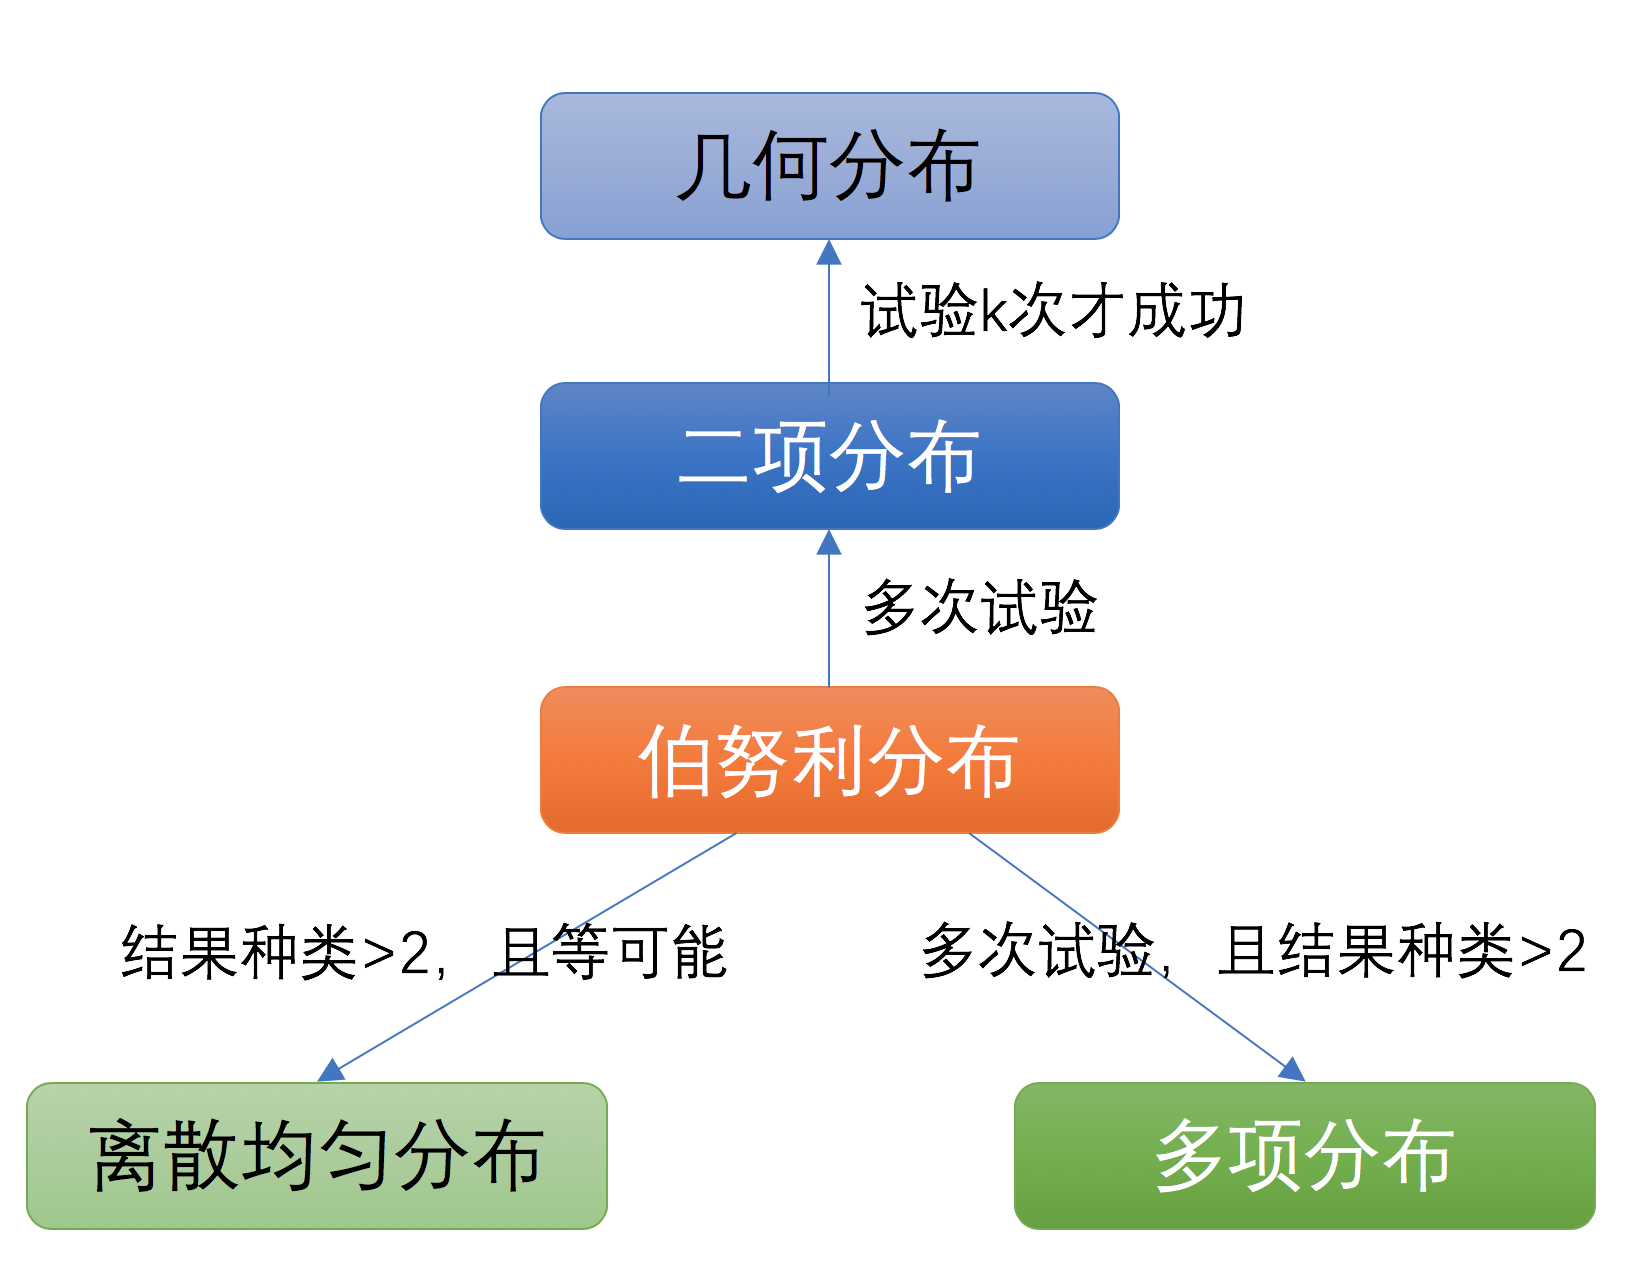
\includegraphics[width=.8\textwidth]{fig/bernoulli_related.png} 
\end{figure}

\subsection{泊松分布}
泊松(Poisson)分布是另外一种很常见的概率分布,由法国数学家西莫恩·德尼·泊松(Siméon-Denis Poisson)在1838年时发表。

我们可以回想一下,生活中很多事情都以特定频率的反复发生的,例如:
\begin{itemize}
    \item 某个医院平均每天有100个新生儿;
    \item 某个客服号码每个小时会接到50个来电;
    \item 某一班公交每个小时会5次经过其中一个站点;
    \item 等等等等;
\end{itemize}

过去发生的平均频度我们是可以计算的,但是我们永远无法精确计算该事件下一次发生的时间点。

泊松分布描述的是:在已知过去发生频率的基础上,预测在接下来一段特定的时间内,该事件发生特定次数的概率。

泊松分布的概率质量函数如下:
$$
P(k) = \frac{e^{-\lambda}\lambda^{k}}{k!} \; ,\lambda \ge 0
$$

这里的$e$是一个常量,约等于2.71828。
$\lambda$是过去单位时间内发生的频率,$k$是预测发生的次数。

我们通过一个具体的例子就很容易理解泊松分布了。

以公交为例,假设我们知道过去它每个小时平均会5次经过其中一个站点($\lambda = 5$),那么接下来的一个小时,它经过的次数很可能是4~6次。不太可能是1次或者10次。我们可以根据概率质量函数,计算它接下来一个小时分别经过1次,4次,5次,10次的概率。

\begin{itemize}
\item 当 $k=1$ 时,$P(1) = \frac{e^{-5}5^1}{1!} \approx 0.034$
\item 当 $k=4$ 时,$P(4) = \frac{e^{-5}5^4}{4!} \approx 0.175$
\item 等等
\end{itemize}

泊松分布的期望值和方差都是$\lambda$。

期望的推导过程:
\begin{align}
E(X) &= \sum_{k=0}^{\infty}k\frac{e^{-\lambda}\lambda^{k}}{(k-1)!} \\
&= \lambda e^{-\lambda}\sum_{k=1}^{\infty}\frac{\lambda^{k-1}}{k!} \\
&= \lambda e^{-\lambda}e^{\lambda} \\
&= \lambda
\end{align}

这里也有一个变换(就是$e^x$的泰勒展开式):
$$
e^{\lambda} = \sum_{k=0}^{\infty}\frac{\lambda^k}{k!}
$$

方差的推导过程:
\begin{align}
E(X^2) &= \sum_{k=0}^{\infty}k^2\frac{e^{-\lambda}\lambda^{k}}{(k-1)!} \\
&= \sum_{k=1}^{\infty}k e^{-\lambda}\lambda \frac{\lambda^{k-1}}{(k-1)!} \\
&= \sum_{k=1}^{\infty}(k-1+1) \lambda e^{-\lambda} \frac{\lambda^{k-1}}{(k-1)!} \\
&= \sum_{k=1}^{\infty}(k-1) \lambda e^{-\lambda} \frac{\lambda^{k-1}}{(k-1)!} + \lambda e^{-\lambda} \sum_{k=1}^{\infty}\frac{\lambda^{k-1}}{(k-1)!} \\
&= \lambda^2 e^{-\lambda} \sum_{k=2}^{\infty}\frac{\lambda^{k-2}}{(k-2)!} + \lambda \\
&= \lambda^2 + \lambda
\end{align} 

$$
D(X) = \lambda^2
$$

\section{连续性分布\cite{Continuous_Variable_Expection_Variation}}
\subsection{高斯分布}
高斯(Gaussian)分布又称正态(Normal)分布。高斯分布的概率密度函数曲线呈钟形,因此人们又经常称之为钟形曲线。高斯分布的概率密度函数和累积分布函数如下图所示:
\begin{figure}[H]
  \centering
  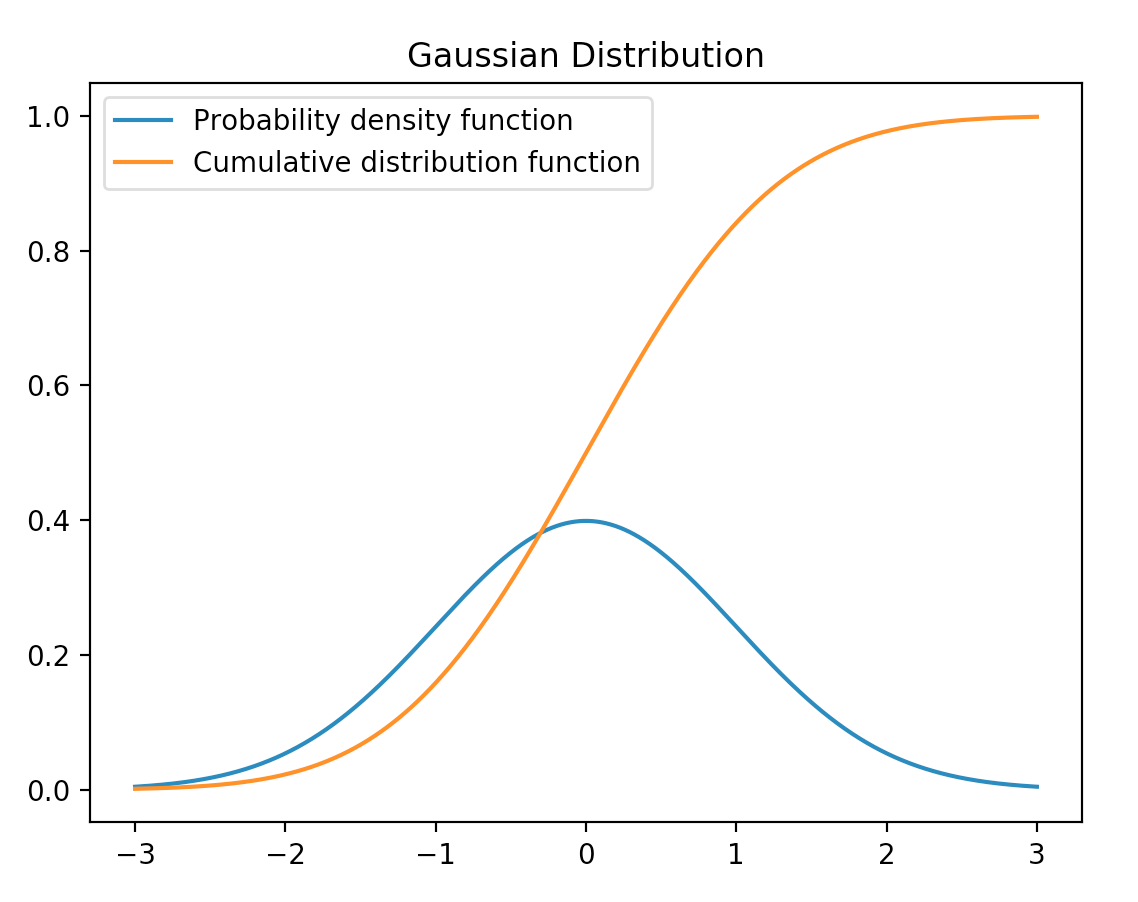
\includegraphics[width=.8\textwidth]{fig/norm_dist.png} 
\end{figure}

从这个图中我们可以看出,对于高斯分布来说,随机变量处于中间的概率是比较大的,而其取非常大或者非常小的值的概率都很小。我们现实中人们的身高,体重,收入等特点都符合这个模型。

高斯分布的概率密度函数如下:
$$
f(x) = \frac{1}{\sqrt{2 \pi}\sigma}e^{-\frac{(x - \mu)^2}{2\sigma^2}}
$$

对于符合高斯分布的随机变量,我们也经常记做下面这样:
$$
X \sim N(\mu, \sigma^2)
$$

在这个函数中,$\mu$决定了高斯分布的中心位置,$\sigma$ 决定了钟型曲线的胖瘦程度。实际上,
$\mu$ 就是高斯分布的期望,而$\sigma^2$就是方差。

当 $\mu = 0, \sigma = 1$时,我们称之为标准正态分布。

期望的推导过程:
\begin{align}
E(X) &= \int_{-\infty}^{+\infty}xf(x)dx \\
&= \frac{1}{\sqrt{2 \pi}\sigma} \int_{-\infty}^{+\infty}xe^{-\frac{(x - \mu)^2}{2\sigma^2}}dx \quad \text{令} \frac{x-\mu}{\sigma} = t \\
&= \frac{1}{\sqrt{2 \pi}}\int_{-\infty}^{+\infty}(\sigma t+\mu)e^{-\frac{t^2}{2}}dt \\
&=  \frac{1}{\sqrt{2 \pi}}\int_{-\infty}^{+\infty}\sigma te^{-\frac{t^2}{2}}dt + \frac{1}{\sqrt{2 \pi}}\int_{-\infty}^{+\infty}{\mu}e^{-\frac{t^2}{2}}dt \quad \text{第一部分为奇函数} \\
&= \frac{1}{\sqrt{2 \pi}}{\mu}{\sqrt{2}}\int_{-\infty}^{+\infty}e^{-(\frac{t}{\sqrt{2}})^2}d{(\frac{t}{\sqrt{2}})} \\
&=  \frac{1}{\sqrt{2 \pi}}{\mu}{\sqrt{2}\sqrt{\pi}} \\
&= \mu
\end{align}

最后一步利用了积分公式:
$$
\int_{-\infty}^{+\infty}e^{-x^2}dx = \sqrt{\pi}
$$

方差的推导过程:
\begin{align}
E(X^2) &= \int_{-\infty}^{+\infty}x^2f(x)dx \\
&= \frac{1}{\sqrt{2 \pi}\sigma} \int_{-\infty}^{+\infty}x^2e^{-\frac{(x - \mu)^2}{2\sigma^2}}dx \quad \text{令} \frac{x-\mu}{\sigma} = t \\
&= \frac{1}{\sqrt{2 \pi}}\int_{-\infty}^{+\infty}(\sigma t+\mu)^2e^{-\frac{t^2}{2}}dt \\
&= \frac{1}{\sqrt{2 \pi}}\int_{-\infty}^{+\infty}({\sigma }^2t^2+2\mu\sigma t+{\mu}^2)e^{-\frac{t^2}{2}}dt \\
&= \cdots \\
&= {\sigma}^2 + {\mu}^2
\end{align}
$$
D(X) = E(X^2) - [E(X)]^2 = {\sigma}^2
$$

\subsection{均匀分布}
均匀(Uniform)分布要简单很多,它指的就是:随机变量在某个区间内,取任意一个值都是等可能的。

其概率密度函数如下:
$$
f(x) = \frac{1}{b-a} , a \le x \le b
$$
很显然,如果我们将这个函数画成图形,那就是两个区间之间的一个水平线。

均匀分布的期望值是$\frac{b+a}{2}$,方差是 $\frac{(b-a)^2}{12}$。

期望的推导过程:
$$
E(X) = \int_a^b\frac{x}{b-a}dx = \frac{1}{b-a}[\frac{1}{2}x^2]_a^b = \frac{b+a}{2}
$$

方差的推导过程:
$$
E(X^2) \int_a^b\frac{x^2}{b-a}dx = \frac{1}{b-a}[\frac{1}{3}x^3]_a^b = \frac{b^2+ab+a^2}{3}
$$
$$
D(X) = E(X^2) - [E(X)]^2 = \frac{(b+a)^2}{12}
$$

\subsection{指数分布}
指数(Exponential)分布是描述泊松过程中的事件之间的时间的概率分布,即事件以恒定平均速率连续且独立地发生的过程。举例来说,如果事件在每个时间点发生的概率相同,那么间隔时间的分布就近似于指数分布。

指数分布的概率密度函数如下:
$$
f(x) = \frac{1}{\lambda}e^{-\frac{x}{\lambda}} \; ,x \ge 0, \lambda > 0
$$

指数分布的期望是 $\lambda$,方差是 $\lambda^2$。

期望的推导过程:

(注:这里指数分布的概率密度函数定义为: $f(x) = {\lambda}e^{-{x}{\lambda}}$)

\begin{align}
E(X) &= \int_0^{+\infty}x{\lambda}e^{-{x}{\lambda}}dx \\
&= -\int_0^{+\infty}xd(e^{-\lambda x}) \\
&= -xe^{-\lambda x}\big|_0^{+\infty} + \int_0^{+\infty} e^{-\lambda x}dx \\
&= -\frac{1}{\lambda}e^{-\lambda x}\big|_0^{+\infty} \\
&= \frac{1}{\lambda}
\end{align}

方差的推导过程:
\begin{align}
E(X^2) &= \int_0^{+\infty}x^2{\lambda}e^{-{x}{\lambda}}dx \\
&= -\int_0^{+\infty}x^2d(e^{-\lambda x}) \\
&= -x^2e^{-\lambda x}\big|_0^{+\infty} + \int_0^{+\infty}2x e^{-\lambda x}dx \\
&= -x^2e^{-\lambda x}\big|_0^{+\infty} + \int_0^{+\infty}2x e^{-\lambda x}dx \\
&= \frac{2}{\lambda} E(X) \\
&= \frac{2}{\lambda^2}
\end{align}
$$
D(X) = E(X^2) - [E(X)]^2 = \frac{1}{\lambda^2}
$$


指数分布的概率密度函数和分布累积函数如下图:
\begin{figure}[H]
  \centering
  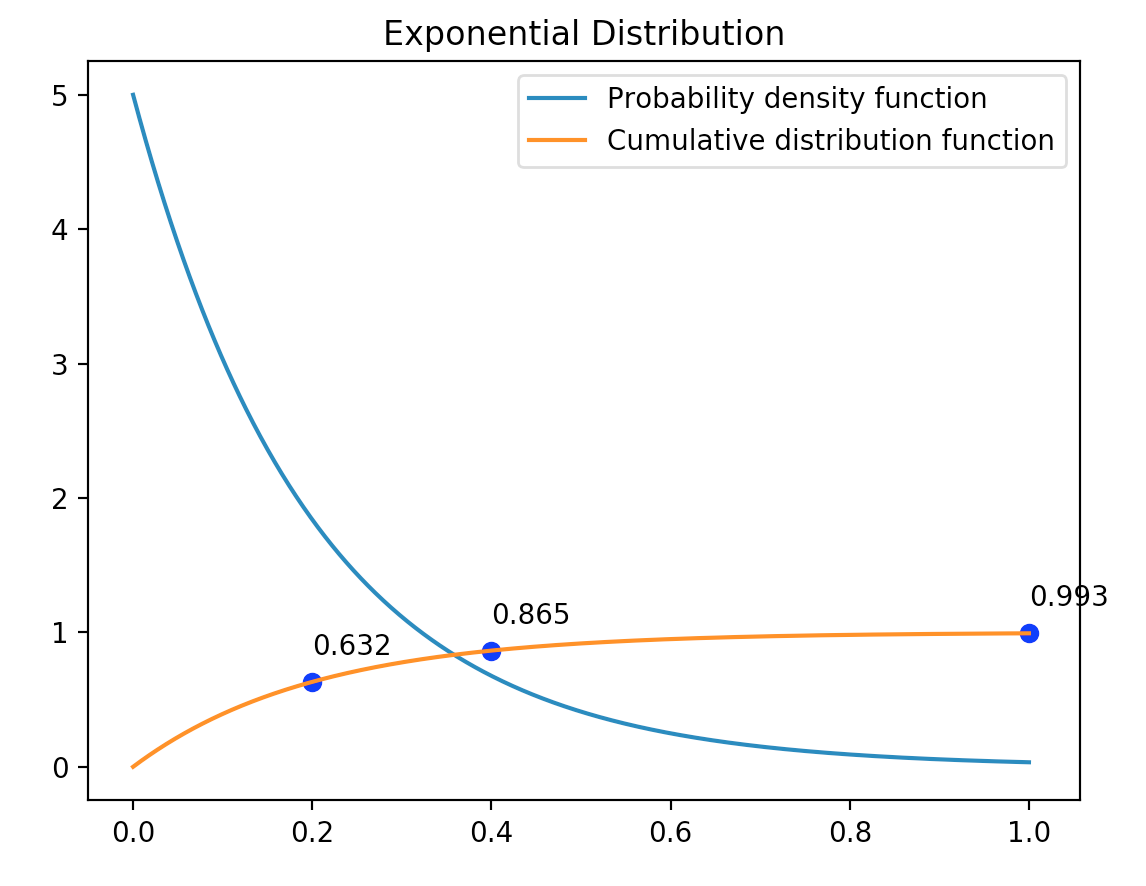
\includegraphics[width=.8\textwidth]{fig/expon_dist.png} 
\end{figure}

我们仍然是以前面提到的公交车为例。假设每个小时某班公交平均有5次会经过其中一个站点。看上图中我们特意在0.2,0.4和1.0这三个点上做的标记。从这个图形中我们可以看出,对于这班公交来说,12分钟(0.2小时)来车的概率是0.632,24分钟(0.4小时)来车的概率是0.865。 当等待的时间越接近一个小时,新的一班车就几乎肯定要来了。

\subsection{帕累托分布\cite{Think_Stats}}
帕累托分布的累积分布函数(CDF)为:
$$
CDF(x) = 1 - (\frac{x}{x_m})^{-\alpha}
$$

其中,参数 $x_m, \alpha$ 决定了分布的位置和形状。$x_m$ 是最小值。

TBD

\subsection{贝塔(Beta)分布}
\subsubsection{一组通俗的解释\cite{Commonly_Understand_Beta_Distribution}}
\textbf{Beta 分布可以看作一个概率的概率分布,当你不知道一个东西的具体概率是多少时,它可以给出了所有概率出现的可能性大小}。

举一个简单的例子,熟悉棒球运动的都知道有一个指标就是棒球击球率(batting average),就是用一个运动员击中的球数除以击球的总数,我们一般认为0.266是正常水平的击球率,而如果击球率高达0.3就被认为是非常优秀的。

现在有一个棒球运动员,我们希望能够预测他在这一赛季中的棒球击球率是多少。你可能就会直接计算棒球击球率,用击中的数除以击球数,但是如果这个棒球运动员只打了一次,而且还命中了,那么他就击球率就是100\%了,这显然是不合理的,因为根据棒球的历史信息,我们知道这个击球率应该是0.215到0.36之间才对啊。

对于这个问题,我们可以用一个二项分布表示(一系列成功或失败),一个最好的方法来表示这些经验(在统计中称为先验信息)就是用 Beta 分布,这表示在我们没有看到这个运动员打球之前,我们就有了一个大概的范围。Beta 分布的定义域是(0,1)这就跟概率的范围是一样的。

接下来我们将这些先验信息转换为 Beta 分布的参数,我们知道一个击球率应该是平均0.27左右,而他的范围是0.21到0.35,那么根据这个信息,我们可以取$\alpha=81, \beta=219$,可以得到如下 Beta 分布的图形:
\begin{figure}[H]
  \centering
  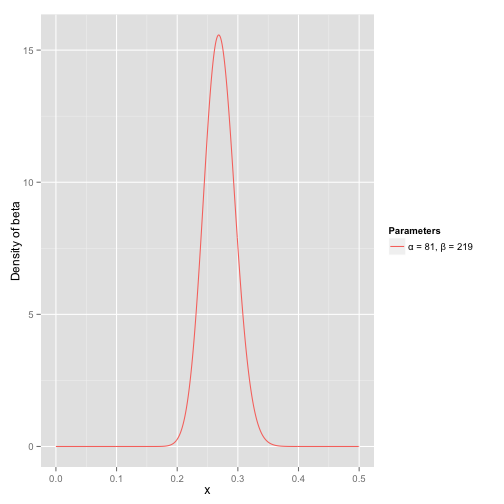
\includegraphics[width=.5\textwidth]{fig/Beta_Distribution_Example_1.png} 
\end{figure}

之所以取这两个参数是因为:;
\begin{itemize}
    \item Beta分布的均值是 $\frac{\alpha}{\alpha+\beta} = \frac{81}{81+219} = 0.27$
    \item 从图中可以看到这个分布主要落在了(0.2,0.35)间,这是从经验中得出的合理的范围。
\end{itemize}

在这个例子里,我们的 x 轴就表示各个击球率的取值,x对应的y值就是这个击球率所对应的概率。也就是说 Beta 分布可以看作一个概率的概率分布。

那么有了先验信息后,现在我们考虑一个运动员只打一次球,那么他现在的数据就是”1中;1击”。这时候我们就可以更新我们的分布了,让这个曲线做一些移动去适应我们的新信息。Beta 分布在数学上就给我们提供了这一性质,他与二项分布是共轭先验的(Conjugate prior)。所谓共轭先验就是先验分布是Beta分布,而后验分布同样是Beta分布。结果很简单:
$$
\text{Beta}(\alpha_0 + \text{hits}, \beta_0 + \text{misses})
$$

其中 $\alpha_0$ 和 $\beta_0$ 是一开始的参数,在这里是81和219。所以在这一例子里,$\alpha$增加了1(击中了一次)。$\beta$没有增加(没有漏球)。这就是我们的新的Beta分布 Beta(81+1,219),我们跟原来的比较一下:
\begin{figure}[H]
  \centering
  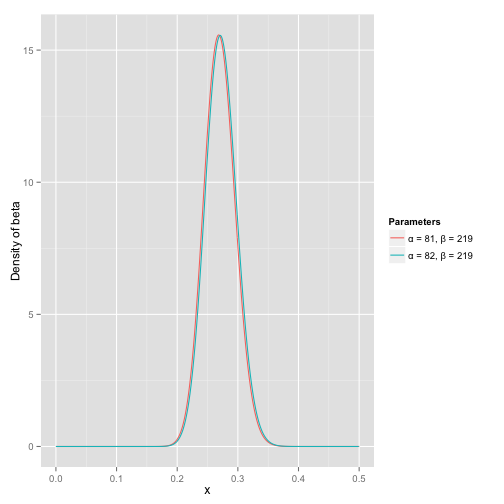
\includegraphics[width=.5\textwidth]{fig/Beta_Distribution_Example_2.png} 
\end{figure}

可以看到这个分布其实没多大变化,这是因为只打了1次球并不能说明什么问题。但是如果我们得到了更多的数据,假设一共打了300次,其中击中了100次,200次没击中,那么这一新分布就是:
$$
\text{Beta}(81+100, 219+200)
$$
\begin{figure}[H]
  \centering
  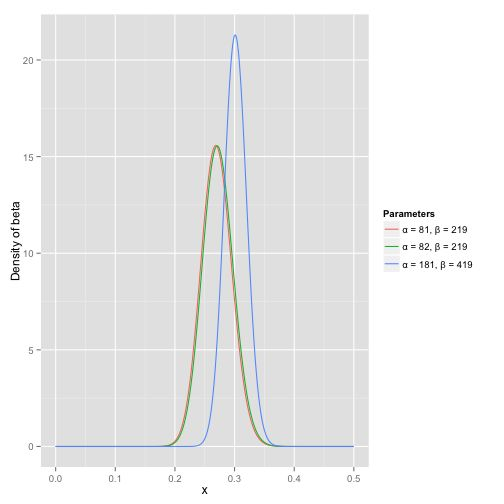
\includegraphics[width=.5\textwidth]{fig/Beta_Distribution_Example_3.jpg} 
\end{figure}

注意到这个曲线变得更加尖,并且平移到了一个右边的位置,表示比平均水平要高。

一个有趣的事情是,根据这个新的 Beta 分布,我们可以得出他的数学期望为:$\frac{\alpha}{\alpha+\beta} = \frac{82+100}{82+100+219+200} = 0.303$,这一结果要比直接的估计要小$\frac{100}{100+200}=0.333$。你可能已经意识到,我们事实上就是在这个运动员在击球之前可以理解为他已经成功了81次,失败了219次这样一个先验信息。

因此,对于一个我们不知道概率是什么,而又有一些合理的猜测时,beta分布能很好的作为一个表示概率的概率分布。

\subsubsection{另一组通俗的解释\cite{Commonly_Understand_Beta_Distribution_Ma}}
\textbf{贝叶斯推断}

各种假设称为先验分布,结合实验数据,推断出后验分布,这就是贝叶斯推断:
$$
\text{先验分布} + \text{实验数据} \Rightarrow \text{后验分布}
$$

\textbf{先验分布}

Beta 分布简记为:Beta(a,b),根据$a, b$参数的不同,Beta分布的形态各异:
\begin{figure}[H]
  \centering
  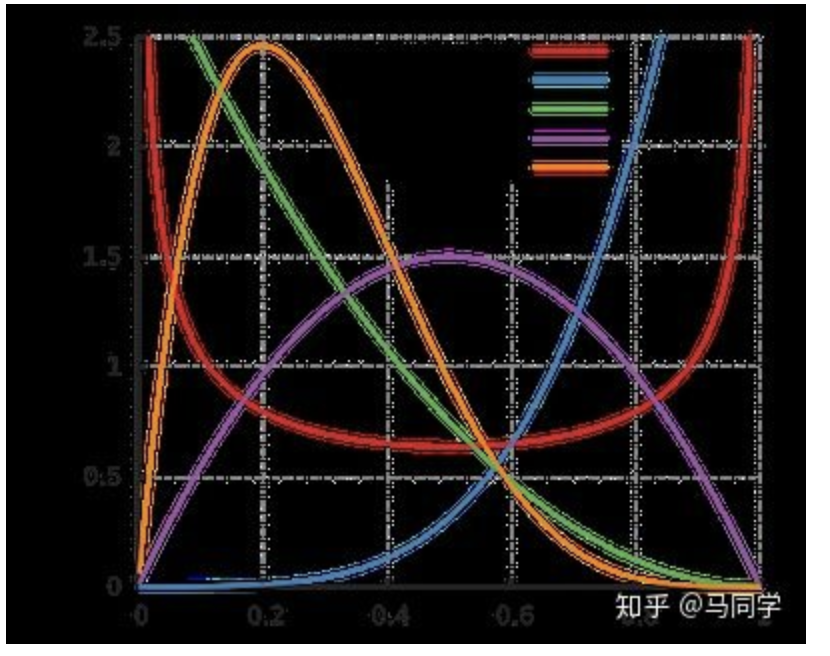
\includegraphics[width=.5\textwidth]{fig/Beta_Distribution_Different_Examples.png} 
\end{figure}

这个特性非常适合用来做先验分布。比如,在韦小宝面前,我们对硬币一无所知。贝叶斯说,一无所知也就是意味着任何概率都是一样的,都是有可能的,所以选用均匀分布
\begin{figure}[H]
  \centering
  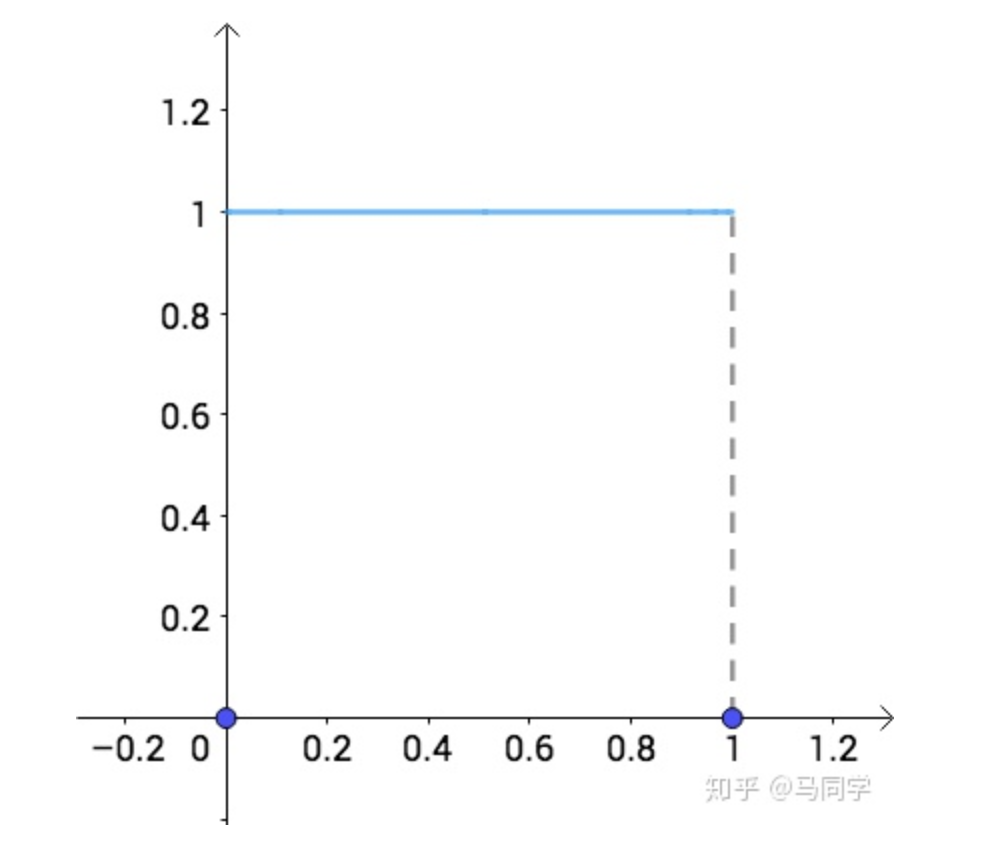
\includegraphics[width=.3\textwidth]{fig/Beta_Distribution_Ma_Example_1.png} 
\end{figure}

Beta(1,1)正好就是均匀分布:
\begin{figure}[H]
  \centering
  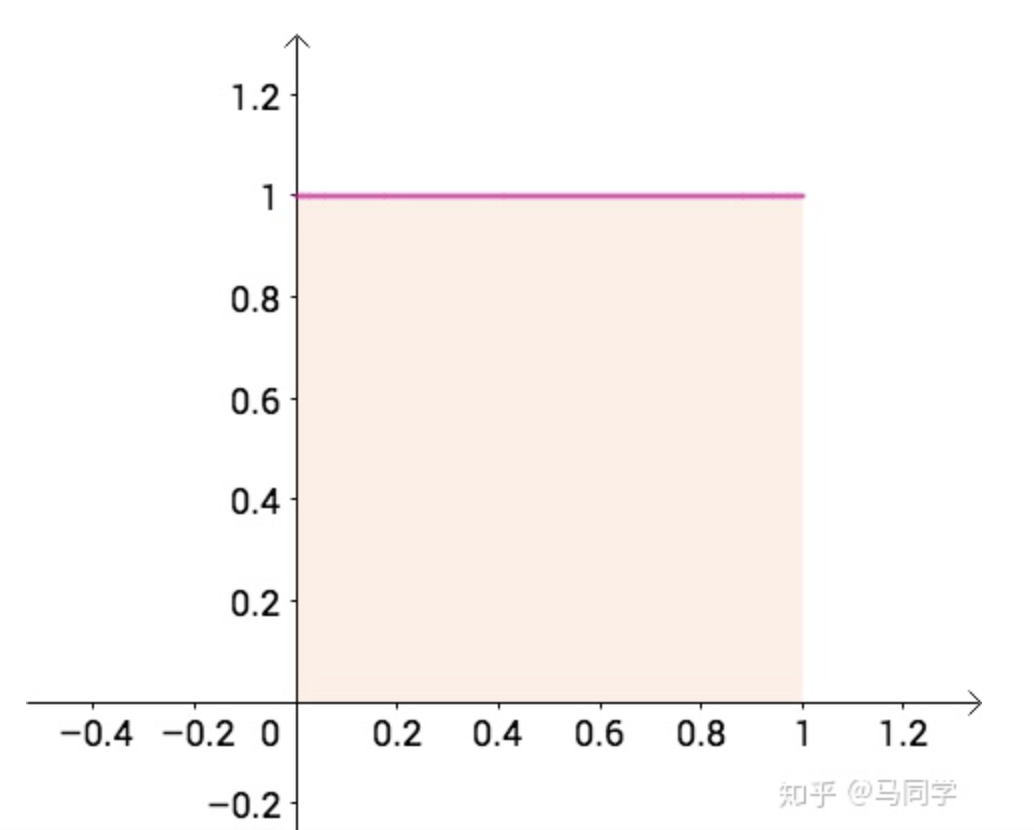
\includegraphics[width=.3\textwidth]{fig/Beta_Distribution_Ma_Example_2.png} 
\end{figure}

正直的陈近南,可能用的是公平硬币,也就是说概率在0、1之间(0表示“字”,1表示“花”),Beta(5,5) 可以表示这样的分布:
\begin{figure}[H]
  \centering
  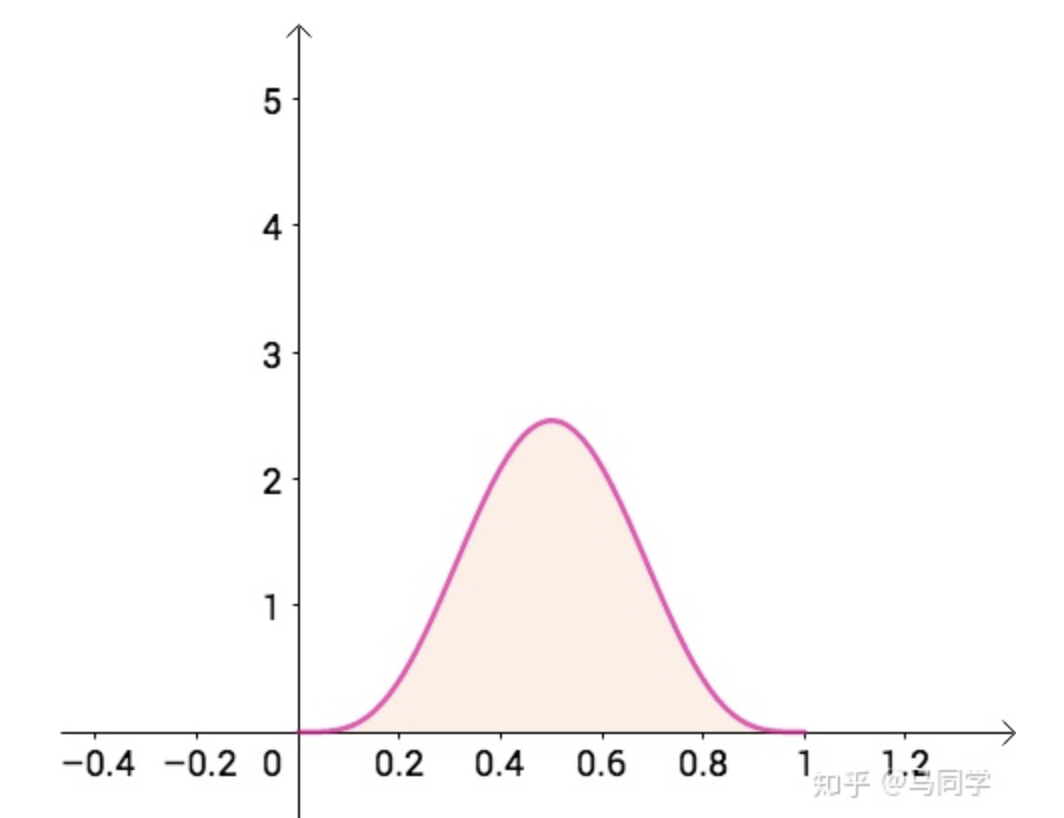
\includegraphics[width=.3\textwidth]{fig/Beta_Distribution_Ma_Example_3.png} 
\end{figure}

而憨坏的多隆,可能用了两面花,也就是说概率可能集中到1附近,Beta(5,1) 可以表示这样的分布:
\begin{figure}[H]
  \centering
  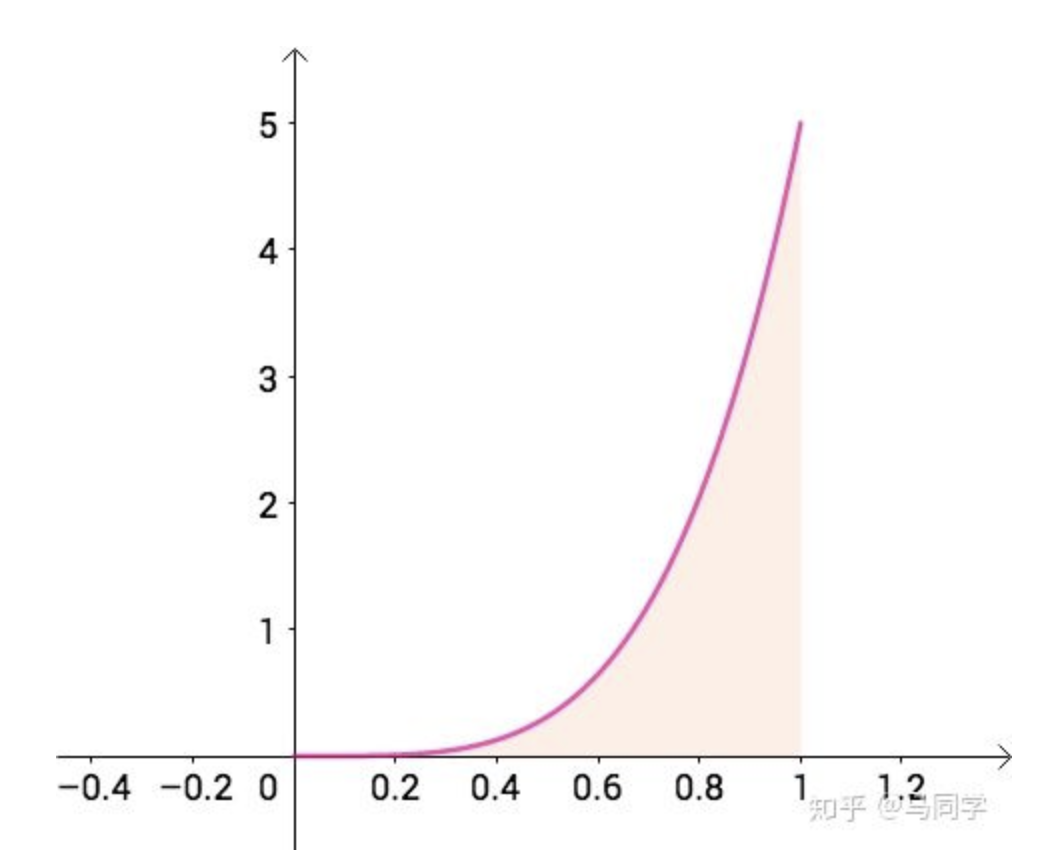
\includegraphics[width=.3\textwidth]{fig/Beta_Distribution_Ma_Example_4.png} 
\end{figure}

也就是说可以用 Beta 分布来模拟各种先验分布:
\begin{itemize}
    \item 一无所知:Beta(1,1)
    \item 公平硬币:Beta(5,5)
    \item 两面花:Beta(5,1)
\end{itemize}

\textbf{后验分布}

用 Beta 分布来模拟扔硬币的先验分布之后,通过贝叶斯推断,得到的后验分布依然是 Beta 分布:
$$
\text{Beta(a,b) + 实验数据} \Rightarrow \textbf{Beta(m,n)} 
$$

具体到抛硬币的例子,就是:
$$
\text{Beta(a,b) + 实验数据} \Rightarrow \textbf{Beta(a+花,b+字)} 
$$

\textbf{代数细节}

贝叶斯推断:
$$
\text{先验分布 + 实验数据} \Rightarrow \textbf{后验分布} 
$$

应用到二项式分布的数学细节如下。假设实验数据$X|p$服从二项分布:
$$
X|p \sim bin(n,p)
$$

上面的式子根据贝叶斯定理(离散贝叶斯可以参看“如何理解贝叶斯定理?”\url{https://link.zhihu.com/?target=https%3A//www.matongxue.com/madocs/279.html},连续贝叶斯可以参看\url{https://link.zhihu.com/?target=https%3A//zh.wikipedia.org/wiki/%25E8%25B4%259D%25E5%258F%25B6%25E6%2596%25AF%25E5%25AE%259A%25E7%2590%2586%23cite_note-2})可以表示为:

$$
\underbrace{f(p|X=k)}_{\text{后验分布}}= \frac{\overbrace{p(X=k|p)}^{\text{实验数据}}\overbrace{f(p)}^{\text{先验分布}}}{\underbrace{P(X=k)}_{\text{常数}}}
$$

其中$k$为“花”的次数。分母与实验数据无关,可以视作常数。因此,写成下面这样更容易看清楚重点:
$$
\underbrace{f(p|X=k)}_{\text{后验分布}} \propto \overbrace{p(X=k|p)}^{\text{实验数据}}\overbrace{f(p)}^{\text{先验分布}}
$$

Beta 分布长成这个样子:
$$
Beta(a,b) = \frac{1}{B(a,b)}x^{a-1}(1-x)^{b-1}
$$

其中,$B$ 为 $Beta$ 函数。随着$a,b$ 的变换,Beta 分布形态各异

\textbf{共轭先验}:\textcolor{red}{对于二项式分布,用 $Beta$ 分布作为先验分布,通过贝叶斯推断之后,后验分布依然是 $Beta$ 分布,这种特性称为共轭先验}。

\subsection{伽马分布}
TBD

\subsection{卡方分布}
TBD

\subsection{柯西分布}
TBD

\subsection{概率密度和卷积\cite{Think_Stats}}
TBD

设两个随机变量 $X$ 和 $Y$ 的累积分布函数分别为 $CDF_X$ 和 $CDF_y$,并且 $Z = X + Y$,那么 $Z$ 服从什么分布呢?

可证明:两个随机变量的和的分布就等于两个概率密度的卷积,即:
$$
PDF_Z = PDF_Y * PDF_X
$$

\section{特征函数}
在概率论中,任何随机变量的特征函数完全定义了它的概率分布。

特征函数定义是:设$X$是实值随机变量,则对任意实数$t$,有:
$$
\phi(t) = Ee^{itX} = E(\cos{(tX)} - i\sin{(tX)}) = E(\cos{(tX)}) + iE(\sin{(tX)})
$$
称为随机变量 $X$ 的特征函数。

(特征函数是概率密度函数的连续傅里叶变换的共轭复数)

\subsection{特征函数为什么叫做特征函数\cite{Why_Called_Feature_Function}\cite{Understand_Feature_Function}}
因为一个分布的特征函数是与该分布密度互相决定的,也就是说,特征函数体现了并蕴含着该分布的全部特征。换言之,随机变量$X$和$Y$同分布,当且仅当它们有相同的特征函数(当然,同时也当且仅当它们有相同的分布密度)。

特征函数是随机变量的分布的不同表示形式。一般而言,对于随机变量 $X$ 的分布,大家习惯用概率密度函数来描述。比如说 $X$ 服从正态分布:$X \sim N(\mu,\sigma)$。

虽然概率密度函数理解起来很直观,但是确实随机变量$X$ 的分布还有另外的描述方式,比如特征函数。

\subsection{泰勒级数}
根据泰勒级数可知,两个函数$f(x)$ 和 $g(x)$ 的各阶导数相等的越多,那么这两个函数越相似。

也即是:
$$
\textbf{各阶导数都相等} \rightarrow f(x) = g(x)
$$

那么,随机变量分布的特征有吗?

\subsection{随机变量分布的特征}
随机变量的特征有如下:
\begin{itemize}
    \item 期望 $\mu$
    \item 方差 $\sigma^2$
    \item 偏态 $Skewness$
    \item 峰态 $Kurtosis$
    \item ……
\end{itemize}

这些特征具体是什么含义就不解释了,说来话长。不过这些特征都跟随机变量的“矩”有关系(什么是“矩”请参考“如何理解概率论中的矩?” )

如期望对应一阶矩,方差对应二阶矩,偏态对应三阶矩等。

直觉上可以有以下推论(其实还是有条件的,这里先忽略这些严格性,在实际应用中如下思考问题不大):

$$
\textbf{各阶矩相等} \rightarrow \textbf{各个特征都相等} \rightarrow \textbf{分布相同} 
$$

\subsection{特征函数}
随机变量 $X$ 的特征函数定义为:
$$
\phi X(t) = E[e^{itX}]
$$
为什么这么定义呢?首先,$e^{itX}$ 的泰勒级数为:
$$
e^{itX} = 1 + \frac{itX}{1!} - \frac{t^2X^2}{2!} + \cdots + \frac{(it)^nX^n}{n!}
$$

代入可以推出:
\begin{align}
\varphi X(t) &= E[e^{itX}] \\
&= E(1 + \frac{itX}{1!} - \frac{t^2X^2}{2!} + \cdots + \frac{(it)^nX^n}{n!}) \\
&= E(1) + E(\frac{itX}{1!}) - E(\frac{t^2X^2}{2!}) + \cdots + E(\frac{(it)^nX^n}{n!}) \\
&= 1 + \frac{it\overbrace{E[x]}^{\text{一阶矩}}}{1!} - \frac{t^2\overbrace{E[x^2]}^{\text{二阶矩}}}{2!} + \cdots +  \frac{(it)^n\overbrace{E[x^n]}^{\text{n阶矩}}}{n!} 
\end{align}
原来特征函数包含了分布函数的所有矩,也就是包含了分布函数的所有特征啊。所以我们可以进一步完善刚才的结论:
$$
\varphi X(t) \textbf{相等} \rightarrow \textbf{各阶矩相等} \rightarrow \textbf{各个特征都相等} \rightarrow \textbf{分布相同} 
$$

所以,特征函数其实是随机变量 $X$ 的分布的另外一种描述方式。

\subsection{特征函数和傅里叶变换的关系\cite{Understand_Feature_Function}}
TBD

\subsection{如何理解概率论中的“矩”?\cite{Understand_Moment_In_Prob}}
对比物理的力矩,你会发现,概率论中的“矩”真的是很有启发性的一个词。

\subsubsection{力矩}
大家应该都知道物理中的力矩,我这里也不展开说细节了,用一幅图来帮助大家回忆一下:
\begin{figure}[H]
  \centering
  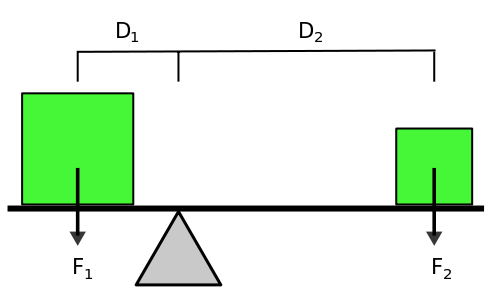
\includegraphics[width=.5\textwidth]{fig/MomentInForce.png} 
\end{figure}
上图中,两边能保持平衡,只要满足下面的式子就可以了(很粗糙的式子,没把力作为向量来考虑):
$$
F_1D_1 = F_2D_2
$$
其中,$F_1D_1$ 和 $F_2D_2$ 都称为力矩。

\subsubsection{概率论中的“矩”}
首先举个彩票的例子:每一注2元,中奖概率分别为:5元:10\%,100元:0.5\%,500万:0.00001\%。

我们用概率来组装一把“秤”:
\begin{figure}[H]
  \centering
  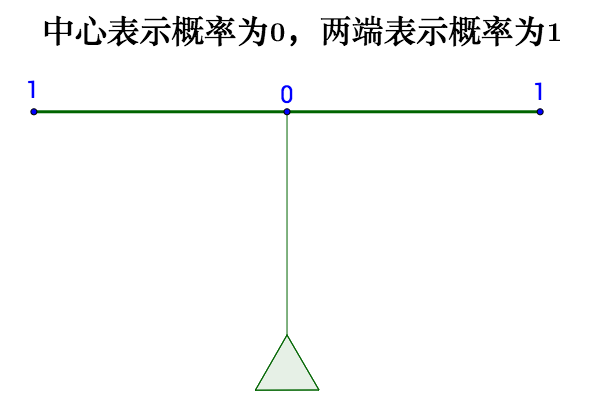
\includegraphics[width=.5\textwidth]{fig/MomentInLottery.png} 
\end{figure}
把整张彩票都放上去称(秤上的刻度是随便画的,因为相差太悬殊,没有办法按照真是比例来画):
\begin{figure}[H]
  \centering
  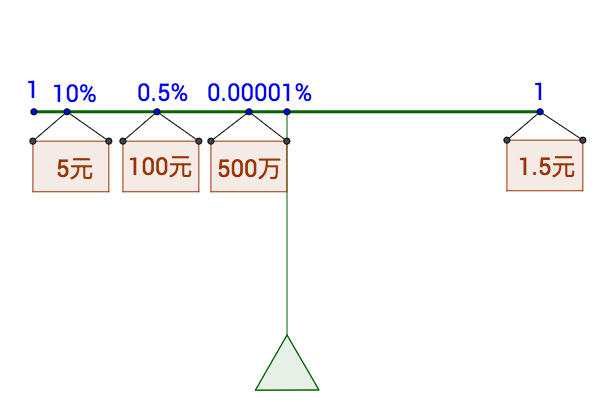
\includegraphics[width=.5\textwidth]{fig/MomentInLottery2.png} 
\end{figure}
$1.5=5\times10\%+100\times0.5\%+5000000\times0.00001\%$ 这张彩票原来只值1.5元?血本无归啊!

\subsubsection{矩}
学过概率的都知道,我们上面计算的就是期望:$E(X) = \sum_ip_ix_i$,其实这就是“矩”,其中:
$$
p_i \quad \textbf{是秤上的刻度}
$$
$$
x_i \quad \textbf{是要称的重量}
$$
因为$x$是一次幂,所以也称为“一阶矩”。

再比如方差:$Var(X) = E[(X-\mu)^2] = \sum_ip_i(x_i-\mu)^2 $

其中的距离$(X-\mu)^2$也需要称量之后才能使用,所以方差也称为“二阶矩”。

“三阶矩”、“四阶矩”、“高阶矩”,各有用途,但是共同的特点就是称量之后才能使用。

\section{正态分布可以生成均匀分布吗}
来源:\url{https://www.zhihu.com/question/25111423/answer/33796836?utm_source=wechat_session&utm_medium=social&utm_oi=38064281878528}

这是阿里的一道笔试题. 假如有一个服从正态分布的真随机数生成器, 是否可以通过程序的处理, 得到一个服从均匀分布的随机数生成器? 如果可以, 具体应该怎样做呢? 

\subsection{均匀分布可以生成正态分布吗}
通常来说我们一般的程序都能更直接地生成均匀分布的随机变量。一种业界广泛使用的做法叫Box-Muller-Wiener算法。首先生成一对$[0,1]$上的均匀分布的,独立的随机变量$A$和$B$。然后用$A *2\pi $作为角度,$sqrt(-2*log(B))$ 作为半径,得到极坐标下的一个点。这个点的两个坐标 $(X,Y)$ 就是一个二维的标准正态分布。

\subsection{正态分布可以生成均匀分布吗}
那么回到本题,如何利用正态分布的两个变量 $X,Y$ 生成均匀分布的随机变量?现有的答案们提到了其中一种做法, 即计算点 $(X,Y)$ 在二维平面内与$x$轴(或任意其他固定方向)的夹角——这样我们就得到了前述过程中的随机变量 $A * 2\pi$。其实另一种方式是计算$exp( -0.5 * (X^2 + Y^2))$ ——这样我们就得到了前述过程中的随机变量$B$。某种意义上来说,后者更为稳定,因为不涉及除法运算(例如$arctan(Y/X)$),可以以很大概率避免 overflow 等等问题。

值得注意的是,点$(X,Y)$到原点距离的平方$X^2 + Y^2$是服从卡方分布的随机变量。当变量数为2的时候,这是一个参数为2的指数分布。对于指数分布的随机变量来说,其累积密度函数有解析的表达式,可以直接通过均匀分布来生成。同样的办法对一维正态分布则只能近似数值处理。

另外一种正确的做法:生成两个独立的正太分布变量$X,Y$, 然后$arctan(X/Y)/(2\pi)+0.5$,可以生成0-1均匀分布的变量,已经通过程序验证。解释下正确性,熟知生成二维标准正态分布的方法就是取两个独立的标准正态分布变量 $X$ 和 $Y$ 放在一起 $(X, Y)$ 就行了,然后\textbf{二维标准正态分布在直角坐标系里有各向同性},也就是 $(X, Y)$这个点所指的方向和 $x$ 轴(或者任何一个给定方向)的夹角是均匀分布的。


%\printbibliography
\bibliography{../ref}
\bibliographystyle{IEEEtran}
\end{document}
